\documentclass[11pt, a4paper]{article}
\usepackage[utf8]{inputenc}
\usepackage[T1]{fontenc}
\usepackage[brazilian]{babel}
\usepackage{amsmath, amssymb}
\usepackage[margin=2.5cm]{geometry}
\usepackage{graphicx}
\usepackage{booktabs}
\usepackage{hyperref}
\usepackage{caption}
\usepackage{float}
\usepackage{xcolor}

\hypersetup{colorlinks=true, linkcolor=blue, urlcolor=cyan}

\title{Latent Fusion --- Resultados Experimentais}
\author{Rodrigo Banin Ferraz de Camargo \\ \texttt{Instituto de Computação -- UNICAMP}}
\date{\today}

\begin{document}
\maketitle

\section{Resumo dos Experimentos}

Este documento registra os resultados experimentais do projeto \textit{Latent Fusion}, que investiga a fusão de embeddings textuais (notícias) com séries temporais financeiras para alocação de portfólio condicionada por regime de mercado.

\subsection{Estrutura do Projeto}

\begin{verbatim}
src/
  backtest/       -- engine, Monte Carlo, grid search, walk-forward, stress tests
  strategy/       -- 8 estratégias (SMA, MeanRev, HMM, VWAP, InstV3, 
                     RegimeRouter, S1Hard70, IntensityGated)
  strategy/trained/ -- modelos treinados com embeddings (Ridge, Lasso, 
                        ElasticNet, MLP, XGBoost)
  features/       -- 23 indicadores técnicos, volatilidade, Hawkes
\end{verbatim}

\section{Estratégias Implementadas}

\subsection{Estratégias Determinísticas}

\begin{itemize}
    \item \textbf{SMA Cross} --- cruzamento de médias móveis (rápida $>$ lenta $\rightarrow$ long)
    \item \textbf{Mean Reversion} --- entrada com z-score $> 1.5$, saída com z-score $< 0.3$
    \item \textbf{HMM Regime} --- 3 estados ocultos (bear/neutral/bull) com re-fit walk-forward
    \item \textbf{VWAP Reversion} --- reversão à média nas bandas de VWAP
    \item \textbf{Institutional V3} --- liquidity sweep + MSB breakout + score multi-fator
    \item \textbf{Regime Router} --- regime de volatilidade roteia entre reversal e momentum
    \item \textbf{S1 Hard70} --- gate de intensidade (embedding drift) + regime router
    \item \textbf{Intensity Gated} --- mesmo que S1 Hard70 com gate soft/hard configurável
\end{itemize}

\subsection{Modelos Treinados com Embeddings}

Modelos supervisionados que aprendem diretamente dos embeddings textuais (SentenceTransformer all-MiniLM-L6-v2, 384 dimensões) para prever retornos forward:

\begin{itemize}
    \item Ridge Regression ($\alpha = 1.0$)
    \item Lasso ($\alpha = 0.001$)
    \item ElasticNet ($\alpha = 0.001$, $l_1 = 0.5$)
    \item MLP Regressor (64, 32 hidden units)
    \item XGBoost (opcional, requer GPU)
\end{itemize}

Redução de dimensionalidade: PCA (32 componentes principais) aplicado após StandardScaler.

\section{Métricas do Backtest Engine}

O engine em \texttt{src/backtest/engine.py} reporta as seguintes métricas para cada backtest:

\begin{itemize}
    \item Retorno total (\%), CAGR (\% anualizado)
    \item Sharpe ratio, Sortino ratio, Calmar ratio
    \item Max drawdown (\%)
    \item CAPM alpha (\% anual), CAPM beta, $R^2$
    \item Buy \& Hold return (\%), excess return (\%)
    \item Win rate (\%), profit factor, número de trades
\end{itemize}

Toda estratégia é comparada automaticamente contra \textbf{buy \& hold} do mesmo ativo no mesmo período. A decomposição alpha/beta segue:

\[
\alpha = \bar{r}_p - \beta \cdot \bar{r}_m, \quad
\beta = \frac{\text{Cov}(r_p, r_m)}{\text{Var}(r_m)}
\]

\section{Estratégia com Embeddings (S1 Hard70)}

A estratégia principal do projeto. Pipeline completo:

\[
\text{notícias} \rightarrow \text{SentenceTransformer} \rightarrow E_t \in \mathbb{R}^{384}
\]
\[
\Delta_t = \|E_t - E_{t-1}\|_2 \rightarrow \text{evento se } \Delta_t \geq P_{95}
\]
\[
\lambda_t = e^{-\beta}\lambda_{t-1} + \alpha \cdot \mathbf{1}_{\text{evento}}, \quad \alpha=0.8, \beta=0.2
\]
\[
\text{gate}_{t,i} = \mathbf{1}\{\text{rank}(\lambda_{t,i}) \geq 0.70\}
\]
\[
\text{signal}_{t,i} = \text{gate}_{t,i} \cdot [R_t \cdot \text{rev}_{t,i} + (1-R_t) \cdot \text{mom}_{3,t,i}]
\]

Onde $R_t$ é o regime de volatilidade (acima/abaixo da mediana), rev é reversal de 1 dia, mom é momentum de 3 dias.

\subsection{Resultado --- Top 50 US Stocks (dados cacheados)}

\begin{table}[H]
\centering
\begin{tabular}{lrrr}
\toprule
Métrica & S1 Hard70 & Buy \& Hold & Excesso \\
\midrule
Retorno (test)   & +122.4\% & +94.3\% & \textbf{+28.1\%} \\
Retorno anual    & 19.05\%  & 15.59\% & +3.46\% \\
Sharpe           & 1.041    & 0.994   & --- \\
Alpha (anual)    & +0.91\%  & ---     & --- \\
Beta             & 1.158    & ---     & --- \\
$R^2$            & 0.983    & ---     & --- \\
\bottomrule
\end{tabular}
\caption{Resultados da estratégia S1 Hard70 com embeddings de texto (50 ativos, top US stocks).}
\end{table}

\begin{figure}[H]
\centering
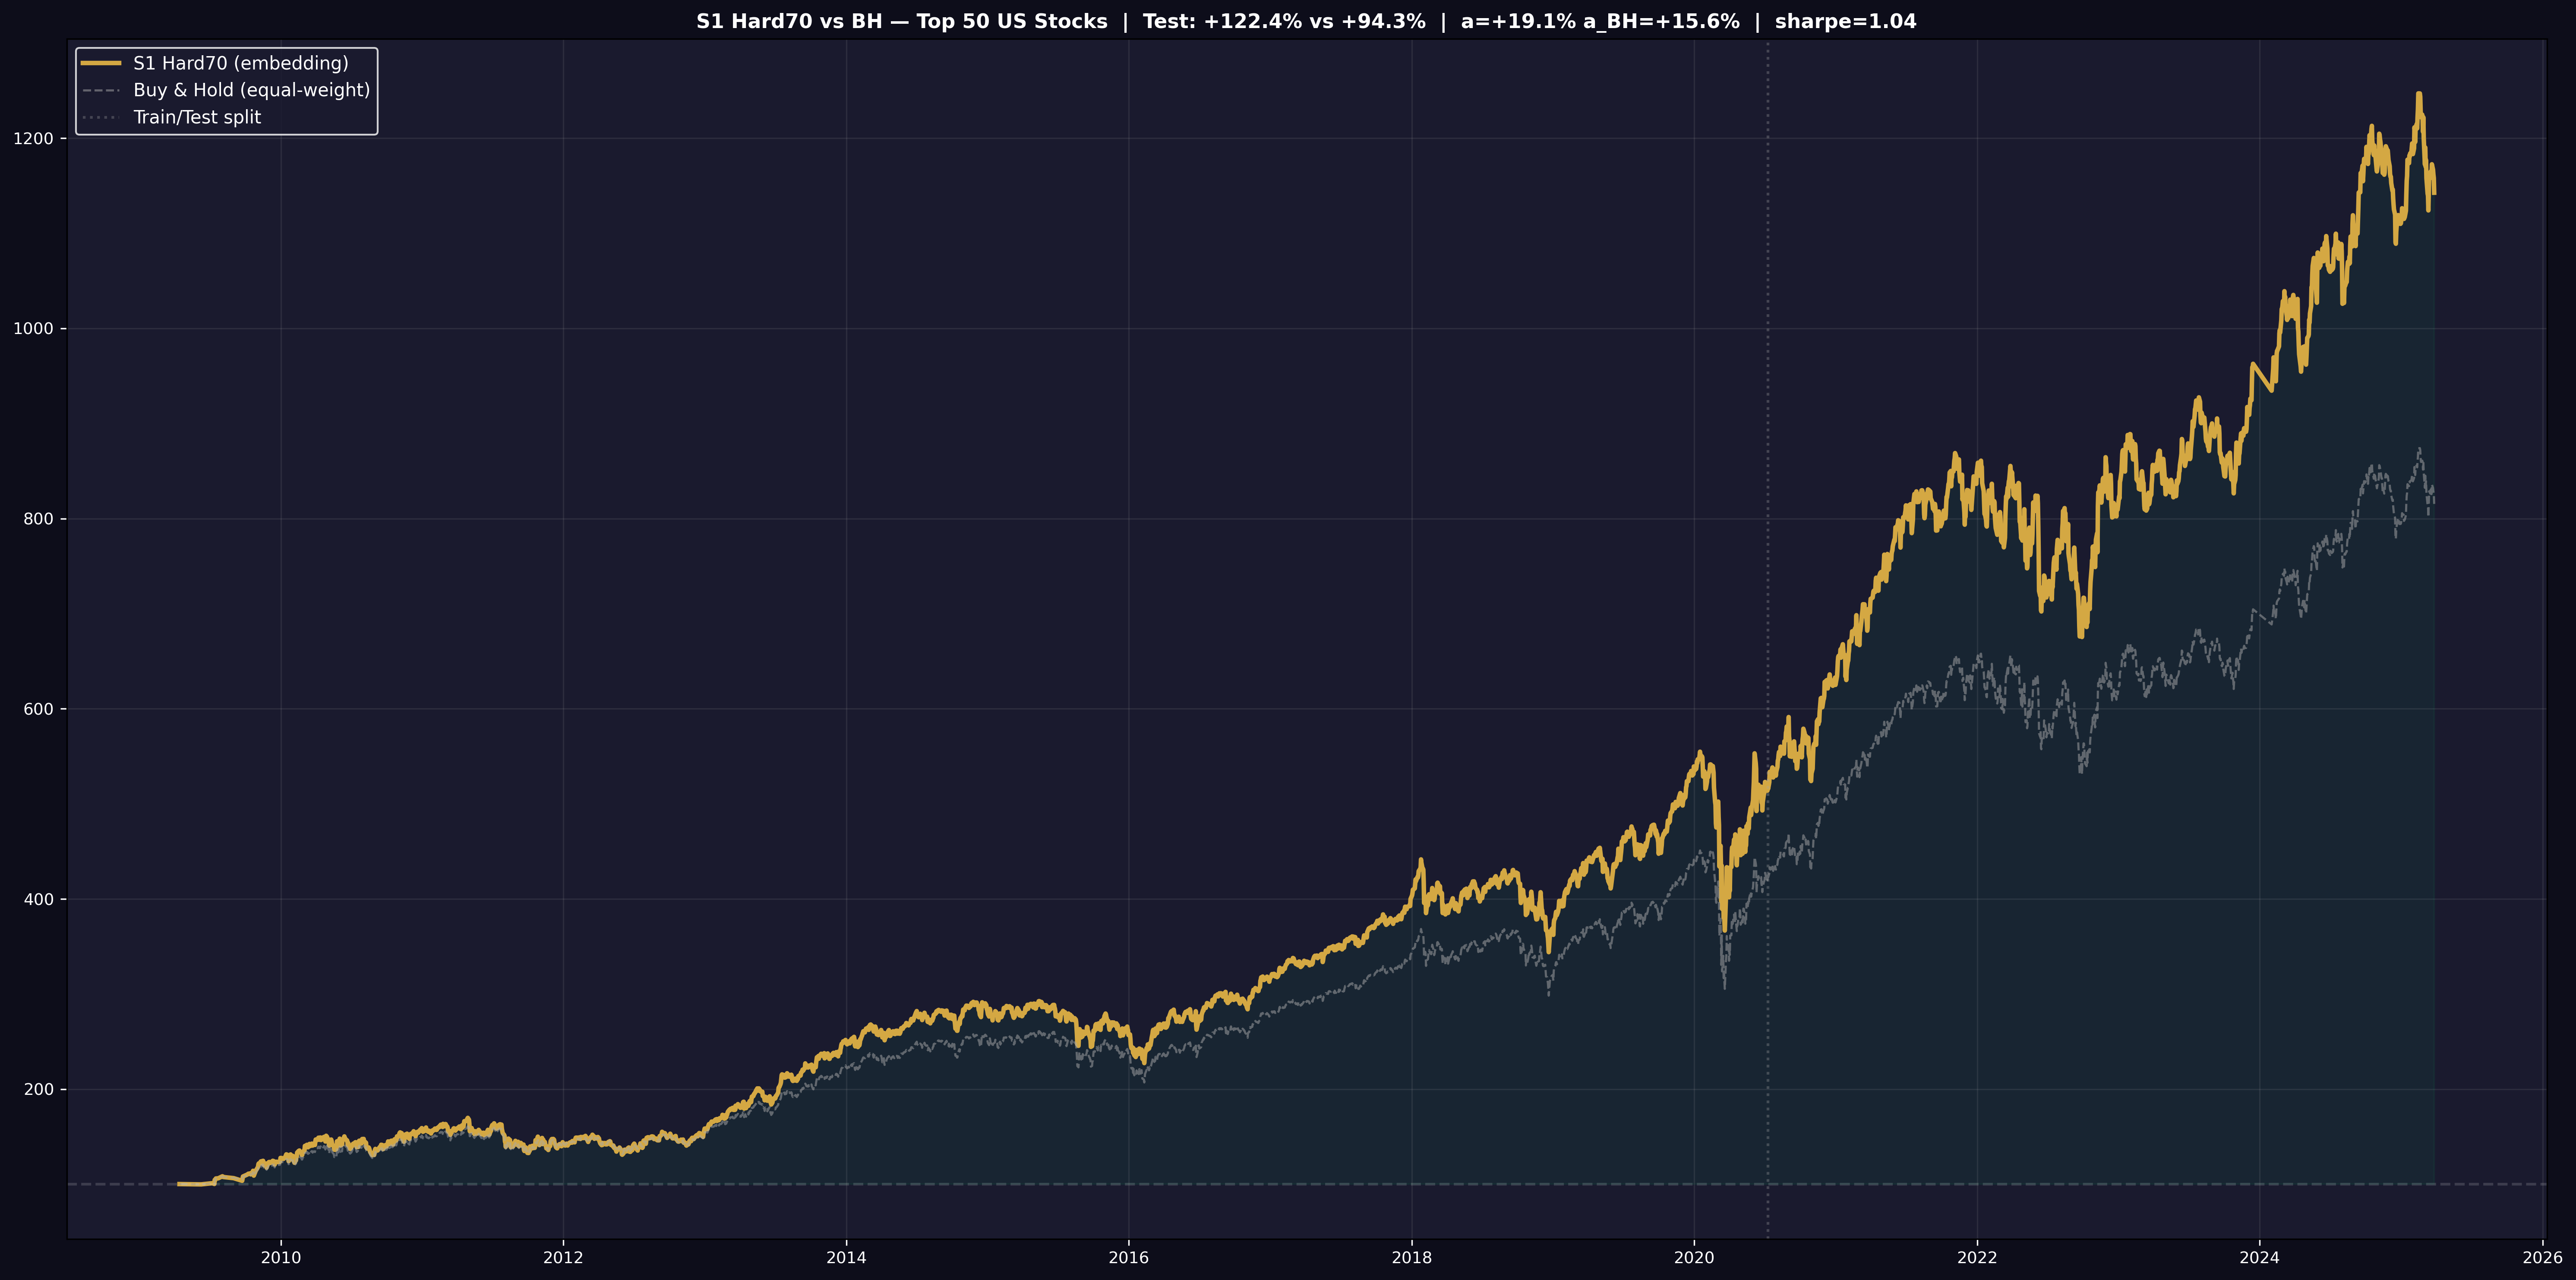
\includegraphics[width=\textwidth]{../images/embedding_strategy_vs_bh.png}
\caption{Curva de equity: S1 Hard70 (embeddings) vs Buy \& Hold.}
\end{figure}

\begin{figure}[H]
\centering
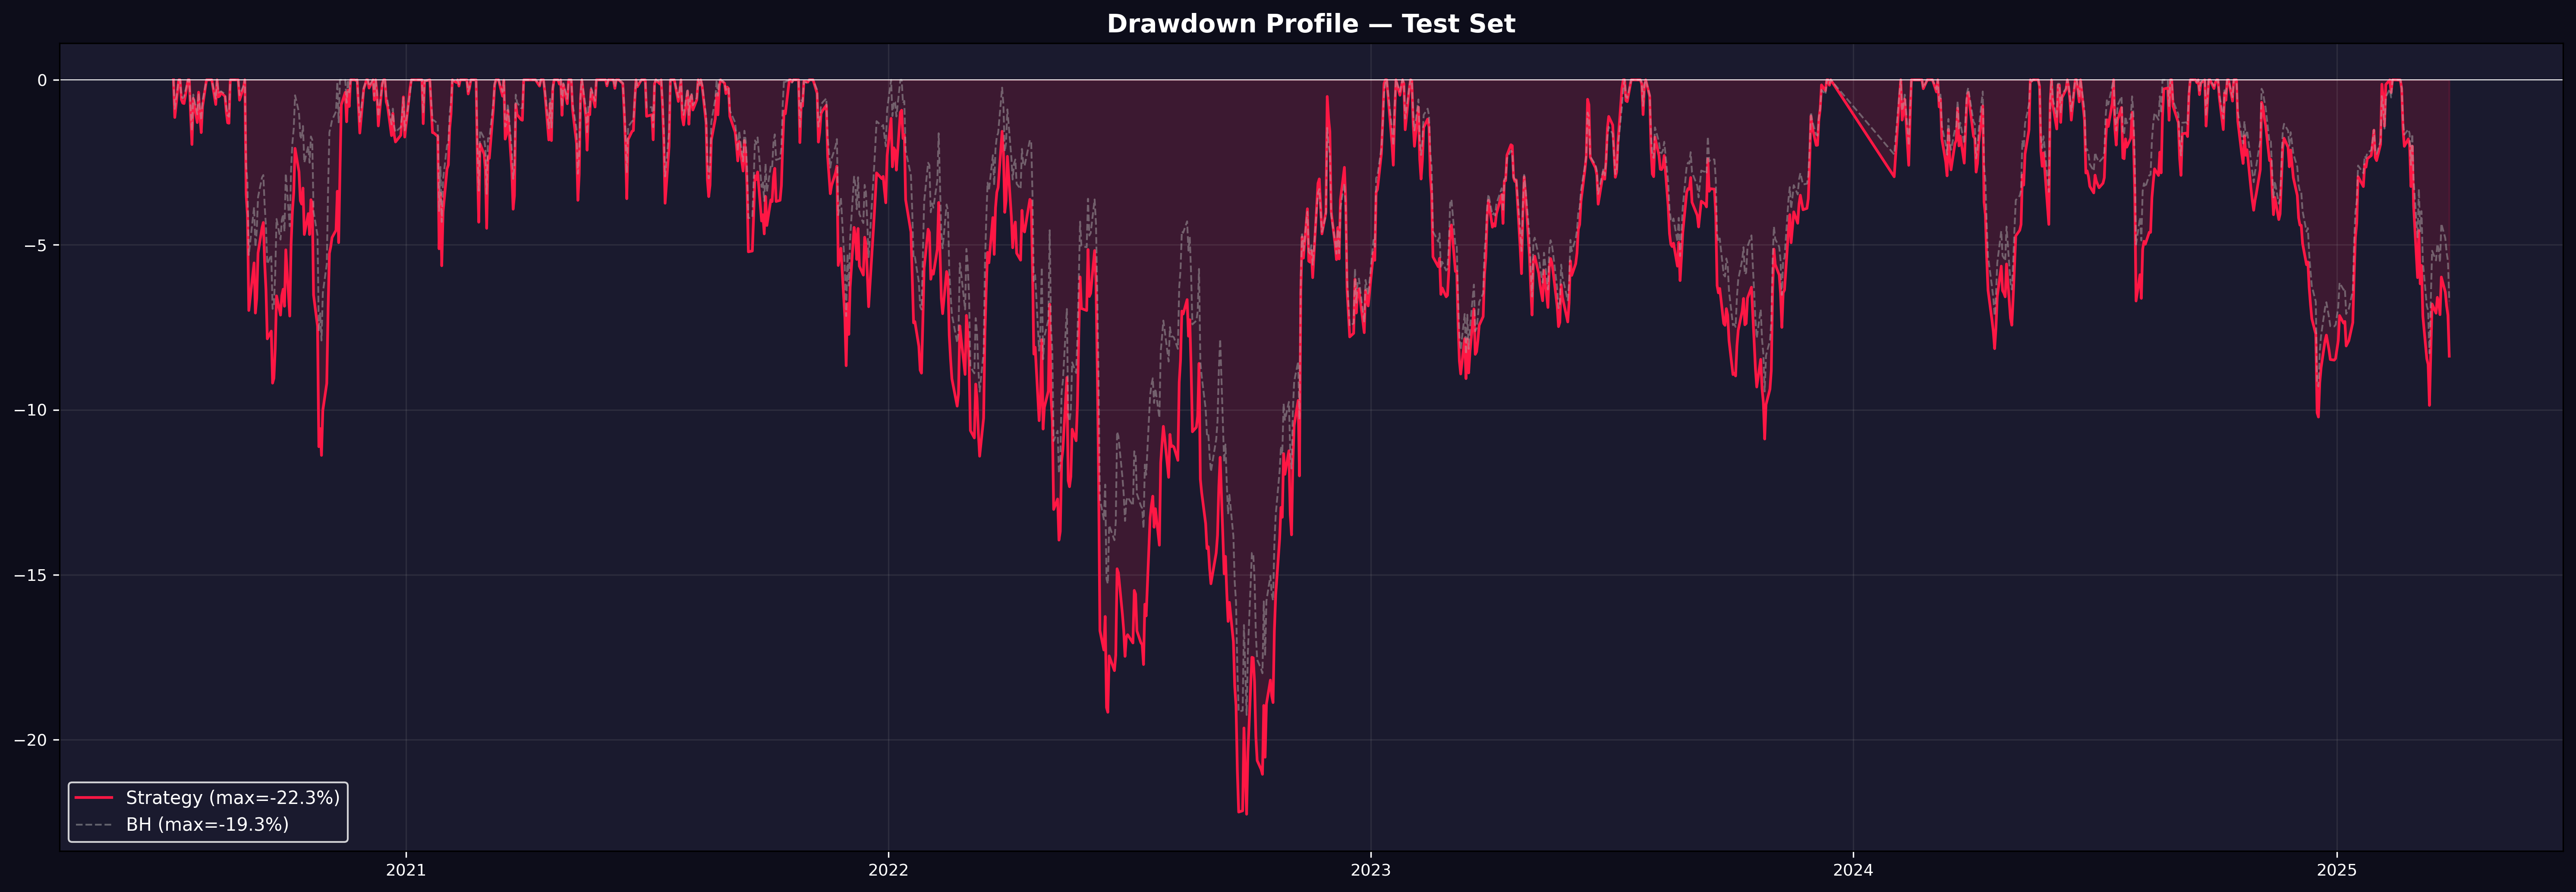
\includegraphics[width=\textwidth]{../images/embedding_strategy_drawdown.png}
\caption{Perfil de drawdown no período de teste.}
\end{figure}

\begin{figure}[H]
\centering
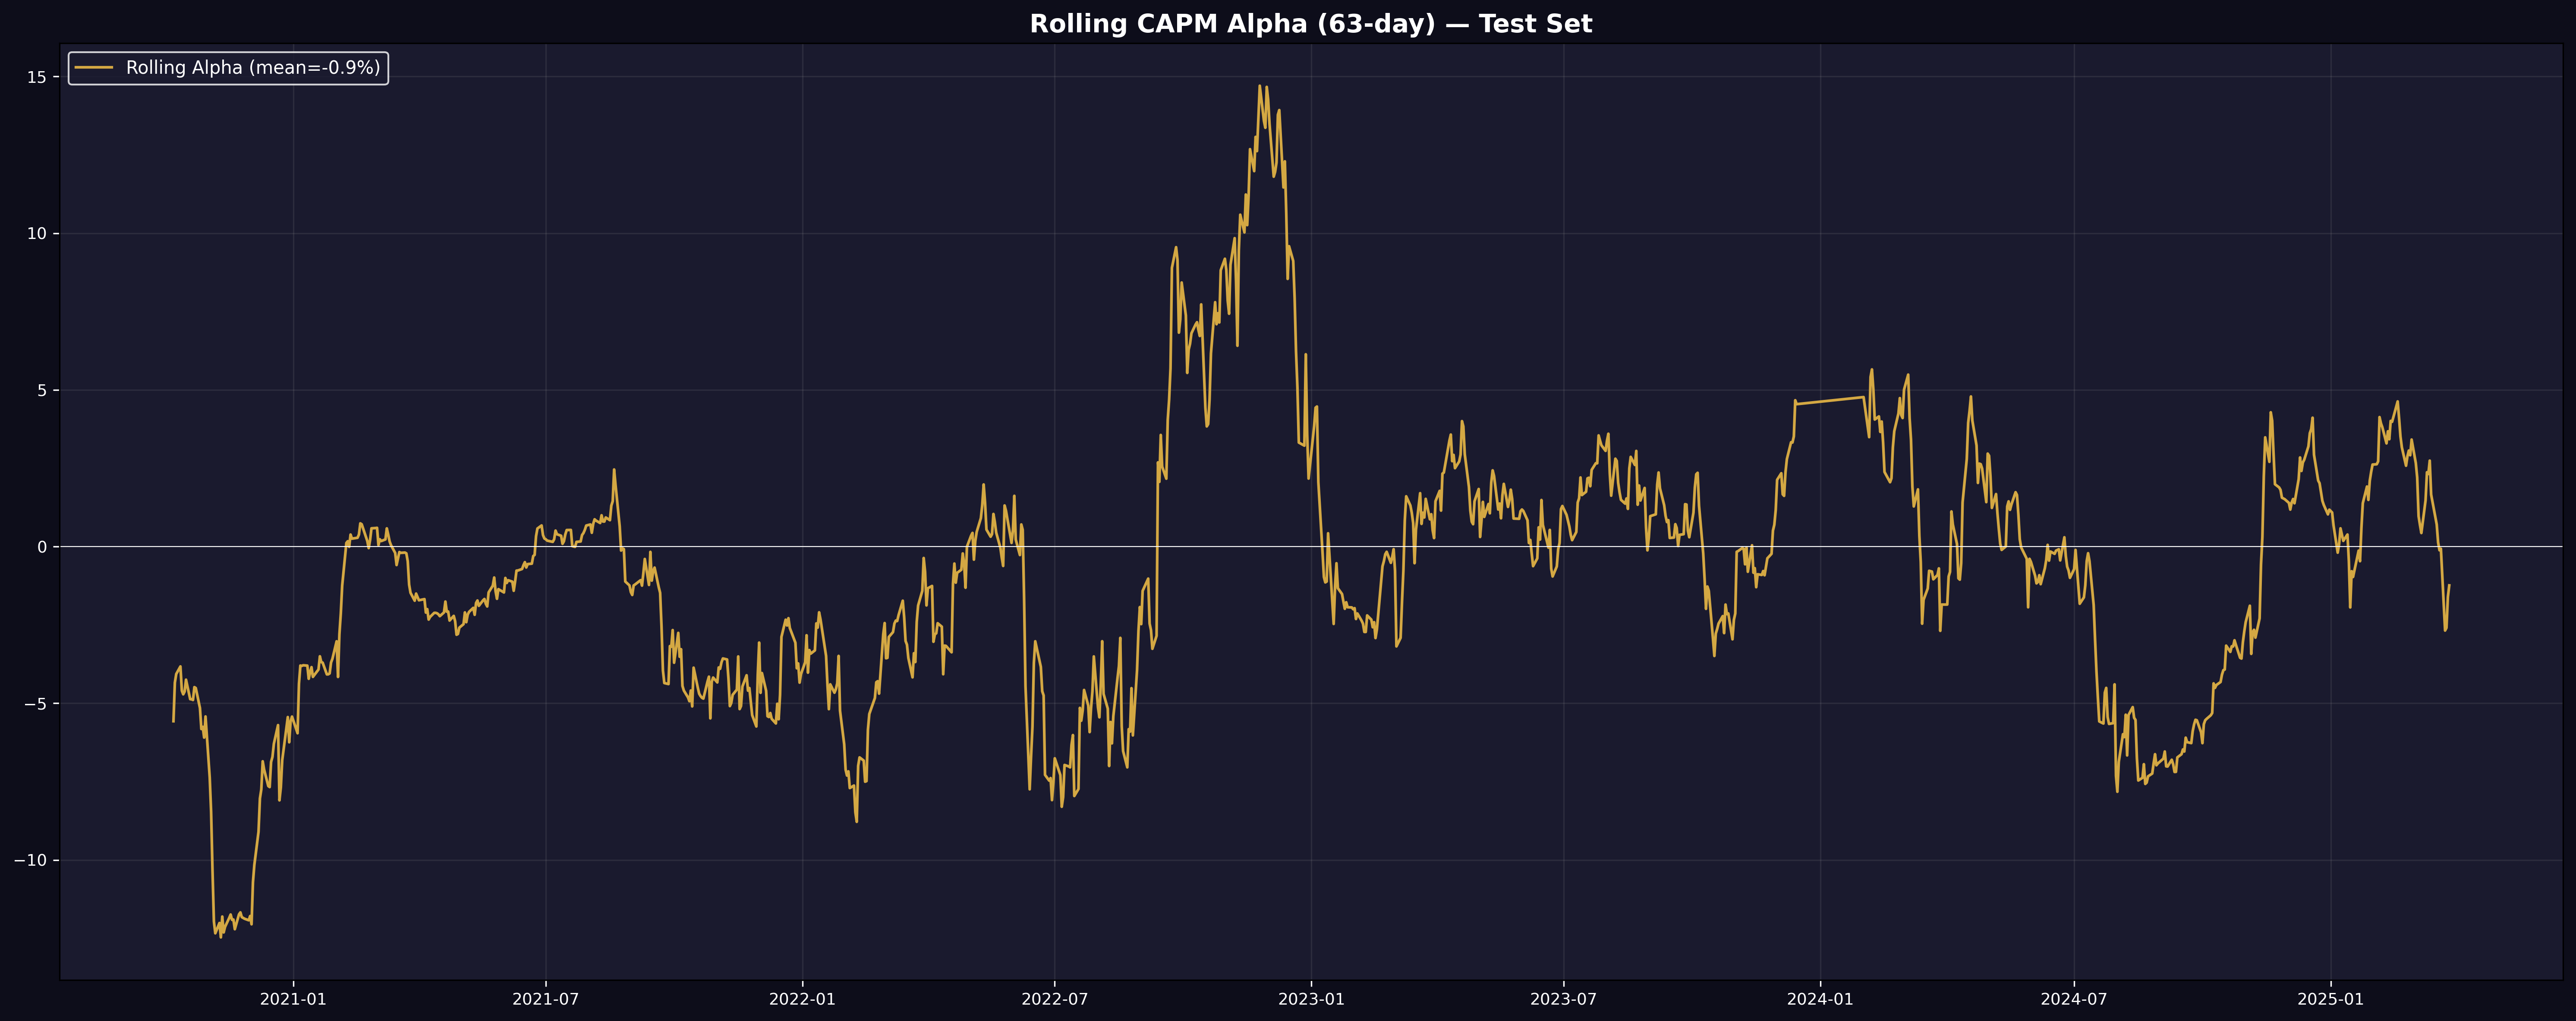
\includegraphics[width=\textwidth]{../images/embedding_strategy_rolling_alpha.png}
\caption{Alpha de CAPM rolling (janela de 63 dias).}
\end{figure}

\section{Comparação Multimodal: Texto vs Numérico}

Duas estratégias rodando no mesmo conjunto de 6 tickers, 2.642 dias:

\begin{itemize}
    \item \textbf{Texto}: SentenceTransformer $\rightarrow$ embedding drift $\rightarrow$ Hawkes $\rightarrow$ S1 Hard70
    \item \textbf{Numérico}: 4 features (vol std, momentum mean, return std, raw return) $\rightarrow$ drift $\rightarrow$ Hawkes $\rightarrow$ S1 Hard70
\end{itemize}

\begin{table}[H]
\centering
\begin{tabular}{lrrrr}
\toprule
Métrica & Texto (S1 Hard70) & Numérico (4-feat) & Buy \& Hold \\
\midrule
Retorno (test) & +5.3\%  & +0.9\%  & +2.8\% \\
Excesso        & \textbf{+2.5\%} & -1.9\% & --- \\
Sharpe         & 0.051   & 0.009  & 0.032 \\
Alpha (anual)  & +1.37\% & -0.01\% & --- \\
Beta           & 1.171   & 1.147  & --- \\
\bottomrule
\end{tabular}
\caption{Comparação entre estratégia com embeddings de texto vs features numéricas.}
\end{table}

\begin{figure}[H]
\centering
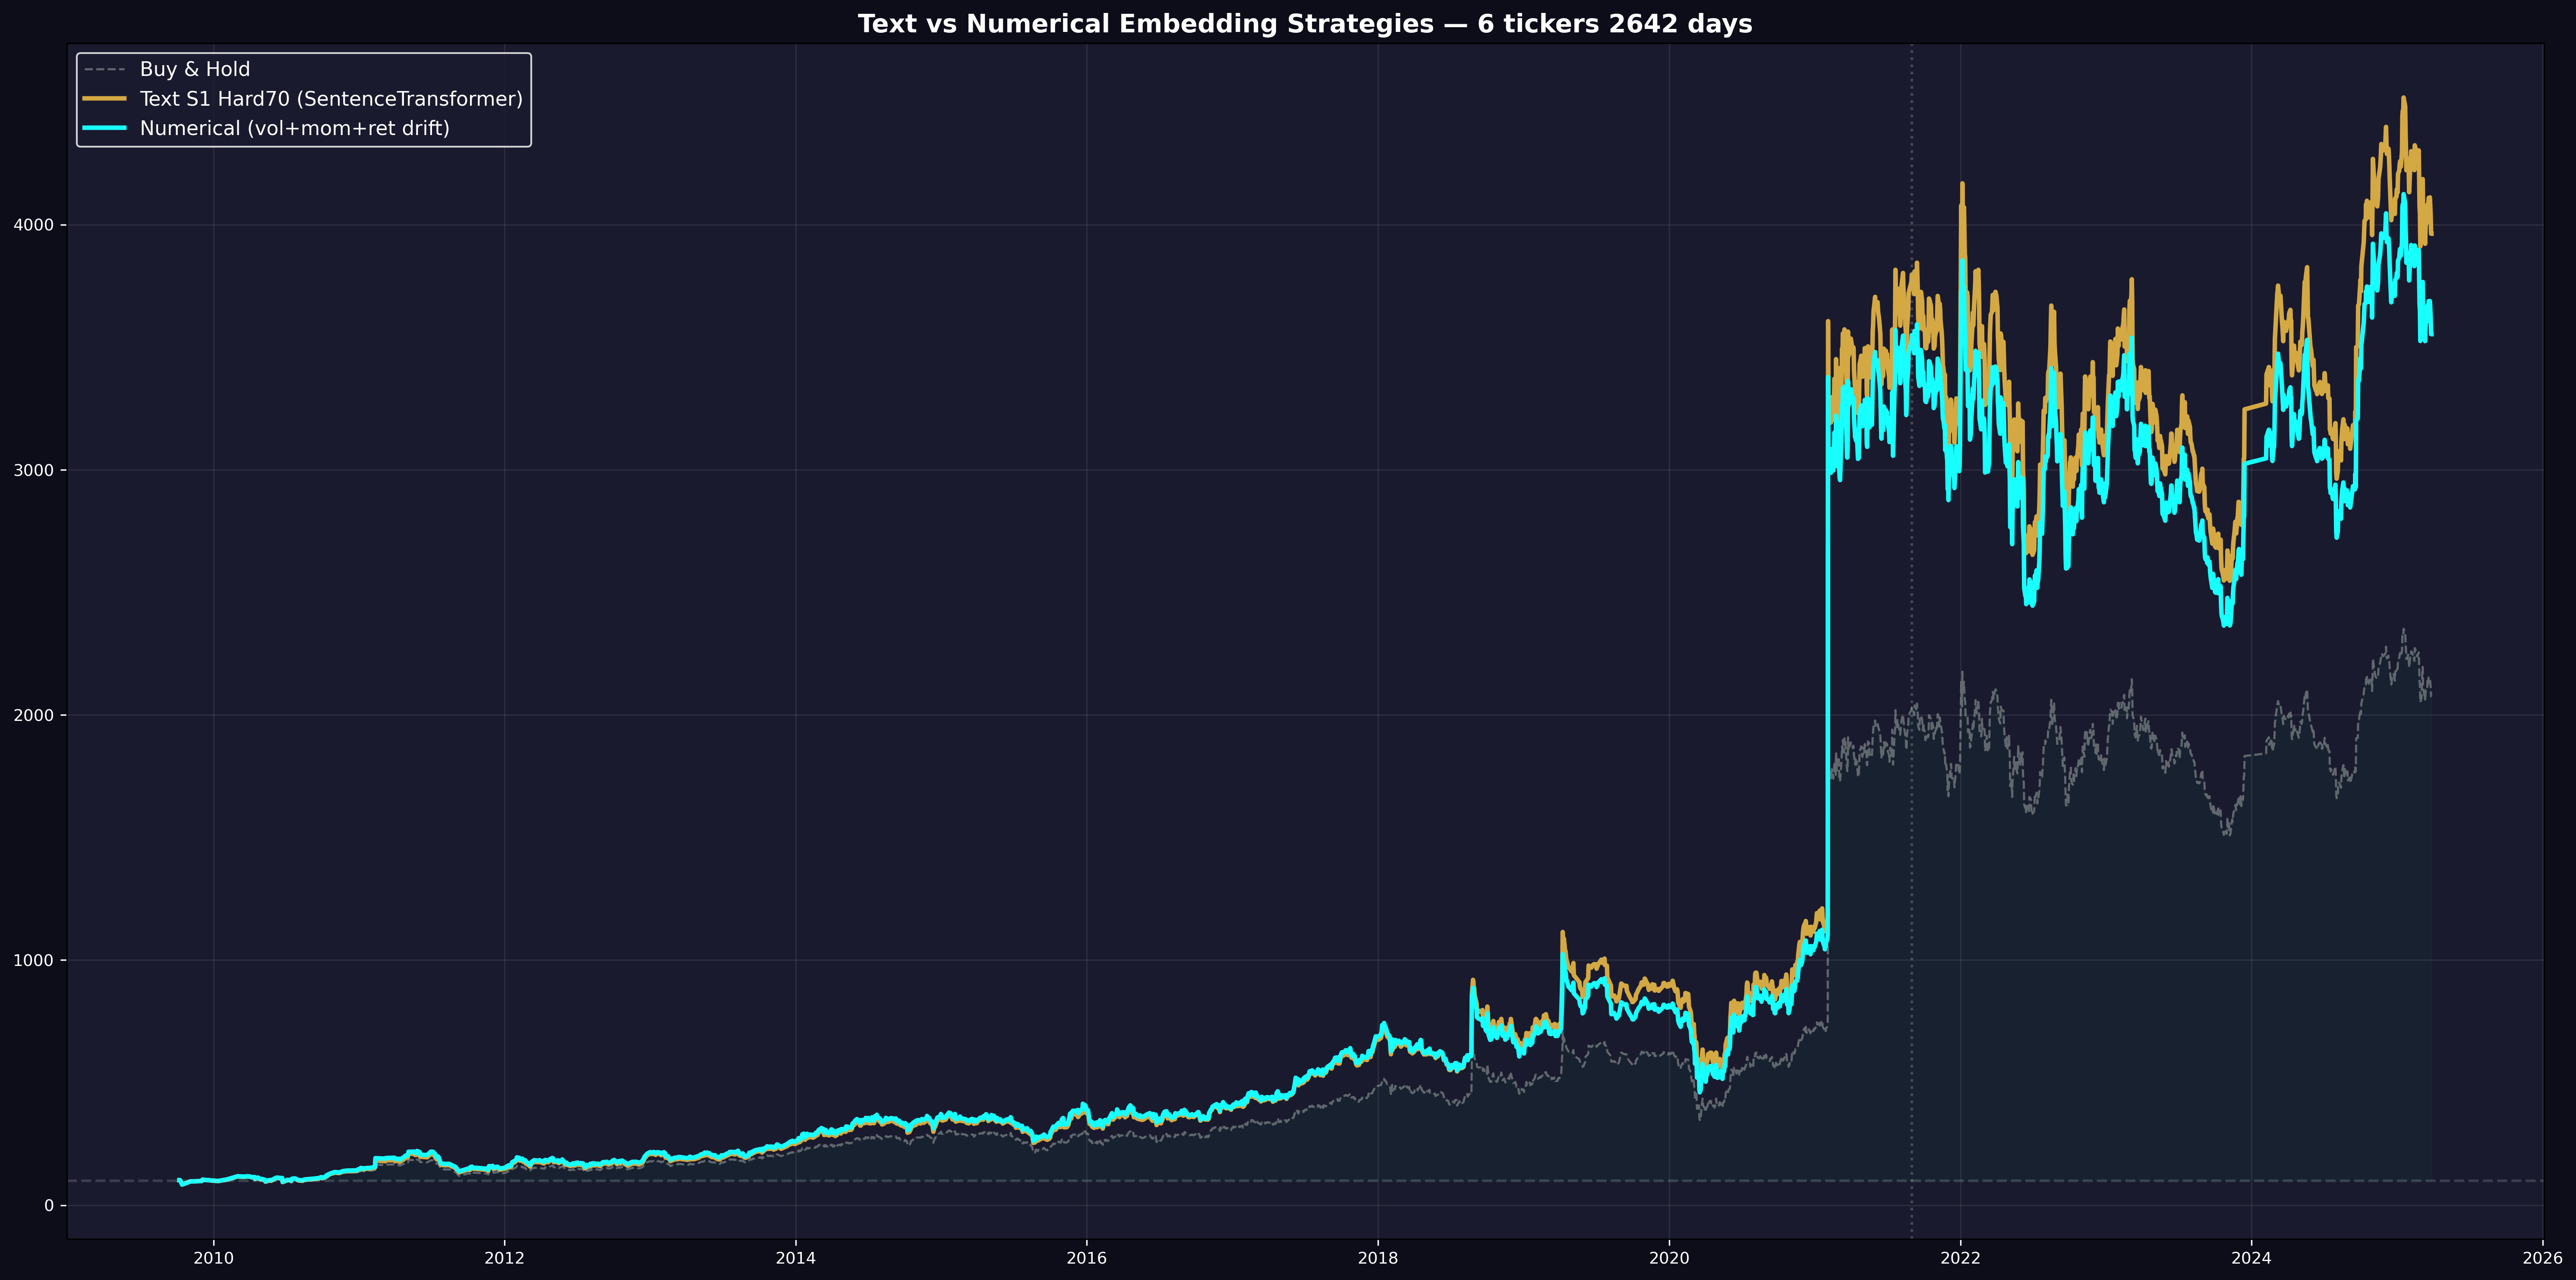
\includegraphics[width=\textwidth]{../images/multimodal_strategies_vs_bh.png}
\caption{Estratégias textuais vs numéricas vs Buy \& Hold.}
\end{figure}

\section{Modelos Treinados com Embeddings}

Quatro modelos de regressão treinados diretamente nos embeddings diários (PCA 32 dimensões) para prever retornos forward. Portfólio cross-sectional com tilt de 5\% ao redor de equal-weight.

\begin{table}[H]
\centering
\begin{tabular}{lrrrrr}
\toprule
Modelo & Corr (treino) & Teste vs BH & Excesso & Sharpe & Alpha \\
\midrule
Ridge      & 0.029 & +116.2\% vs +94.3\% & +22.0\% & 1.000 & +0.28\% \\
Lasso      & 0.015 & +118.7\% vs +94.3\% & \textbf{+24.4\%} & 1.019 & \textbf{+0.57\%} \\
ElasticNet & 0.016 & +118.1\% vs +94.3\% & +23.9\% & 1.015 & +0.51\% \\
MLP (64,32)& 0.112 & +117.9\% vs +94.3\% & +23.7\% & 1.015 & +0.51\% \\
\bottomrule
\end{tabular}
\caption{Modelos treinados com embeddings. Lasso obteve o melhor excesso de retorno e alpha.}
\end{table}

\begin{figure}[H]
\centering
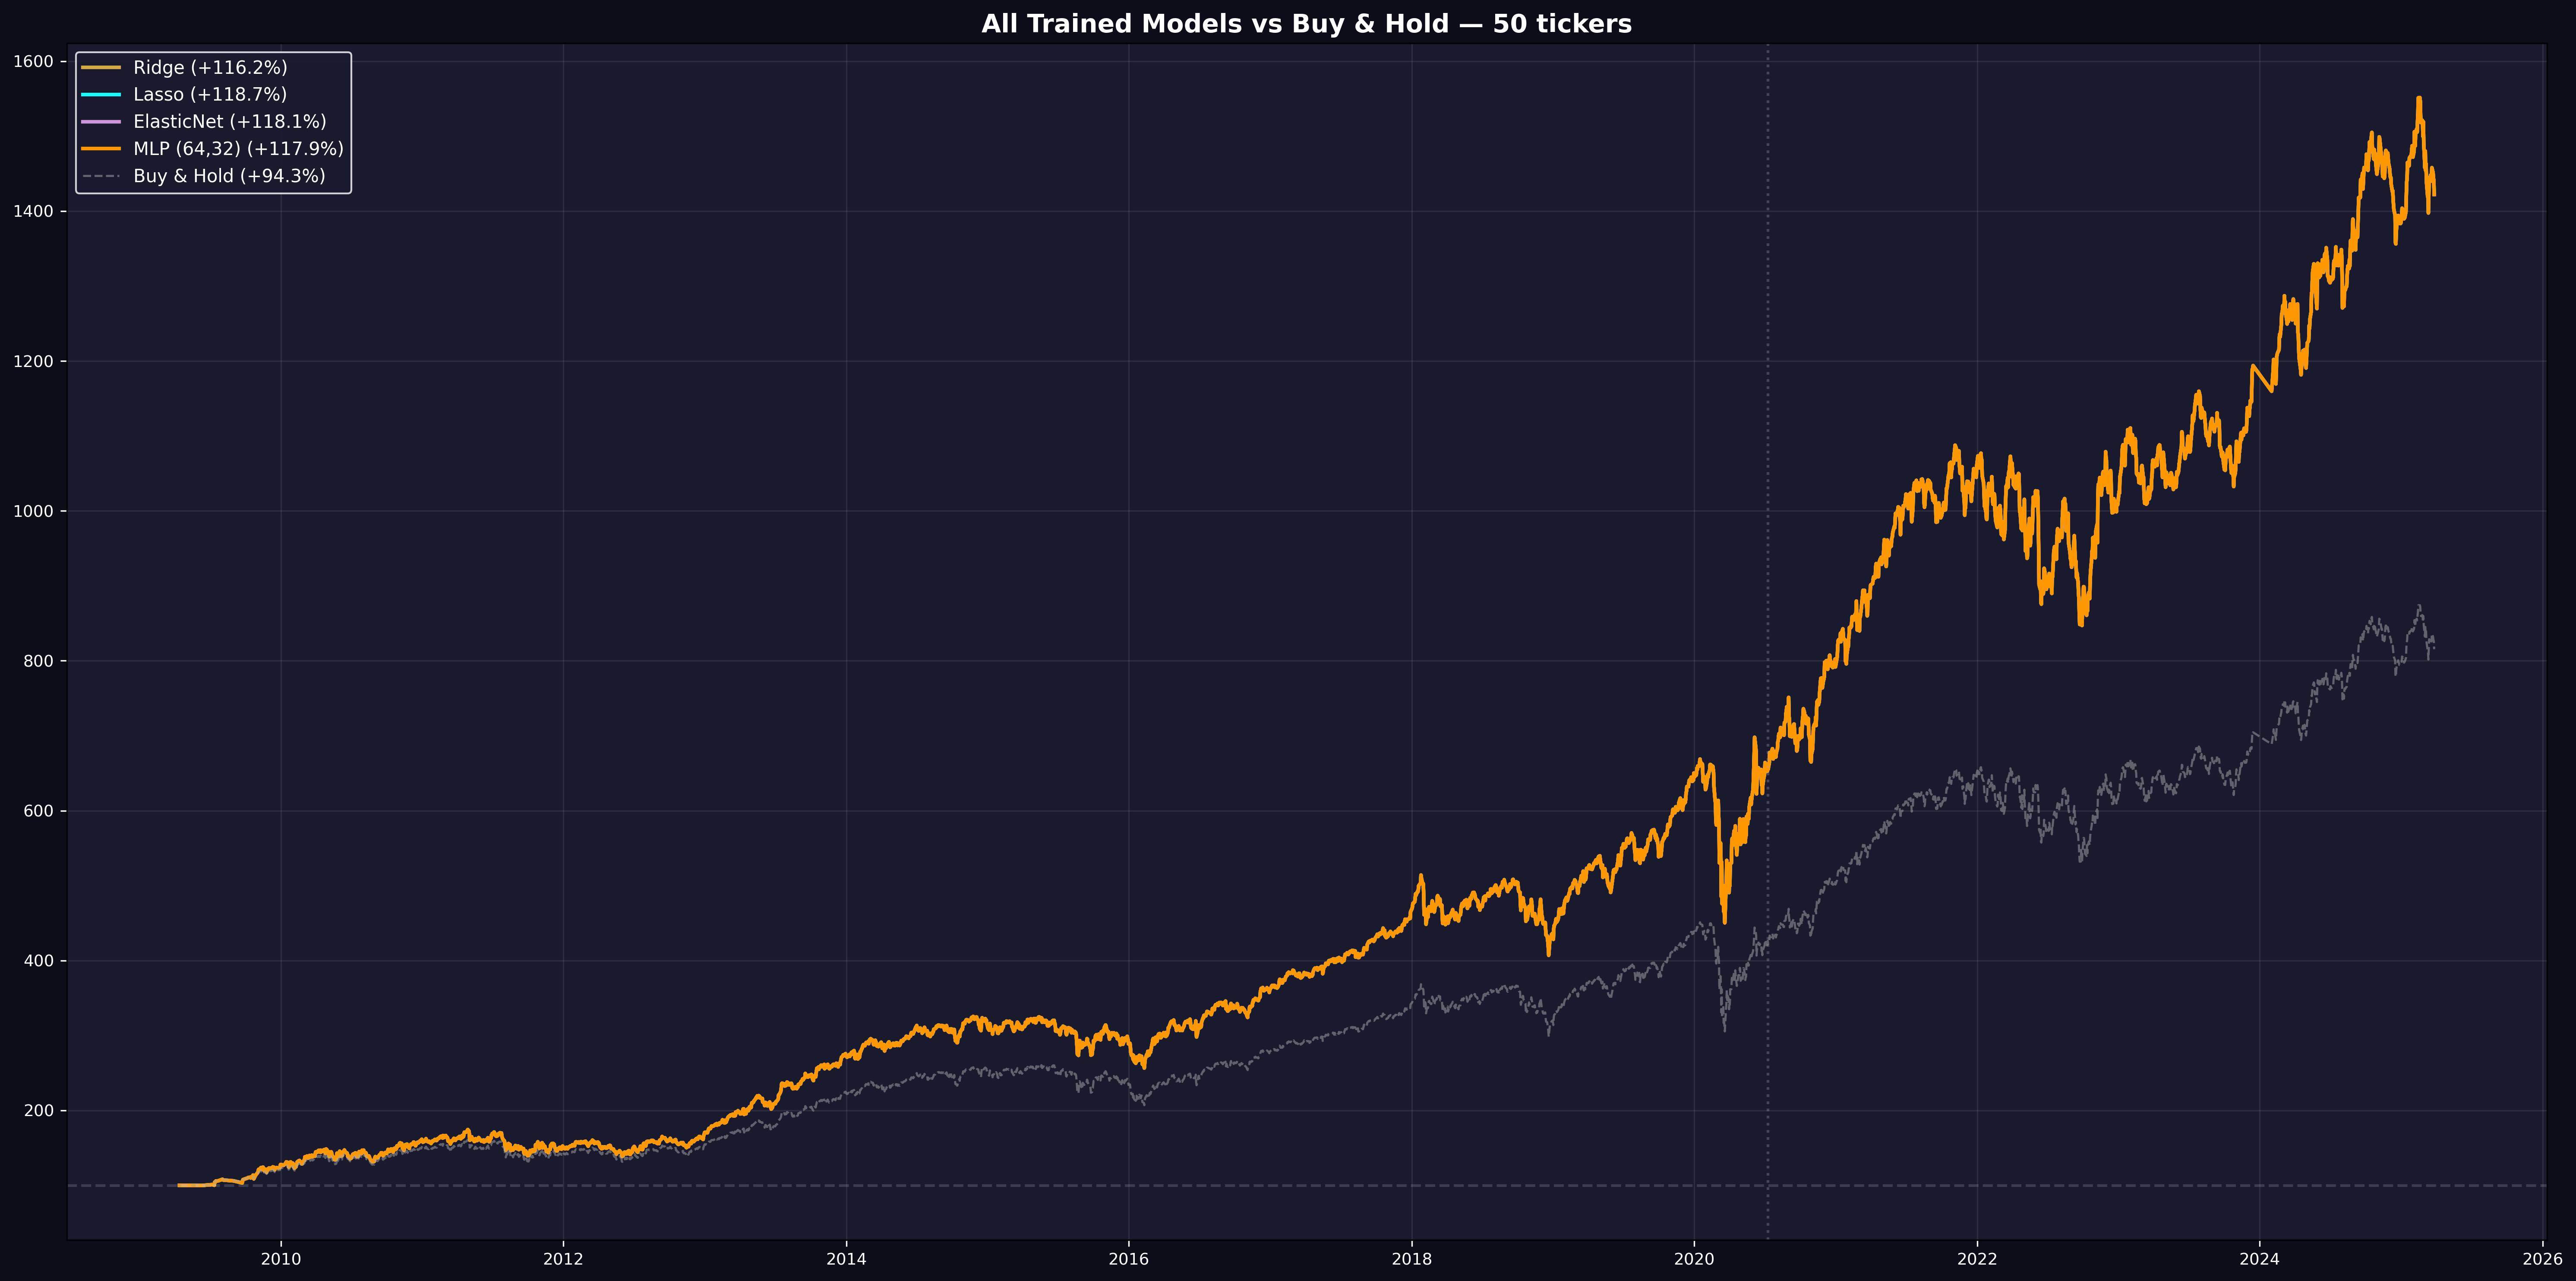
\includegraphics[width=\textwidth]{../src/strategy/trained/images/all_models_vs_bh.png}
\caption{Curvas de equity de todos os modelos treinados vs Buy \& Hold.}
\end{figure}

\begin{figure}[H]
\centering
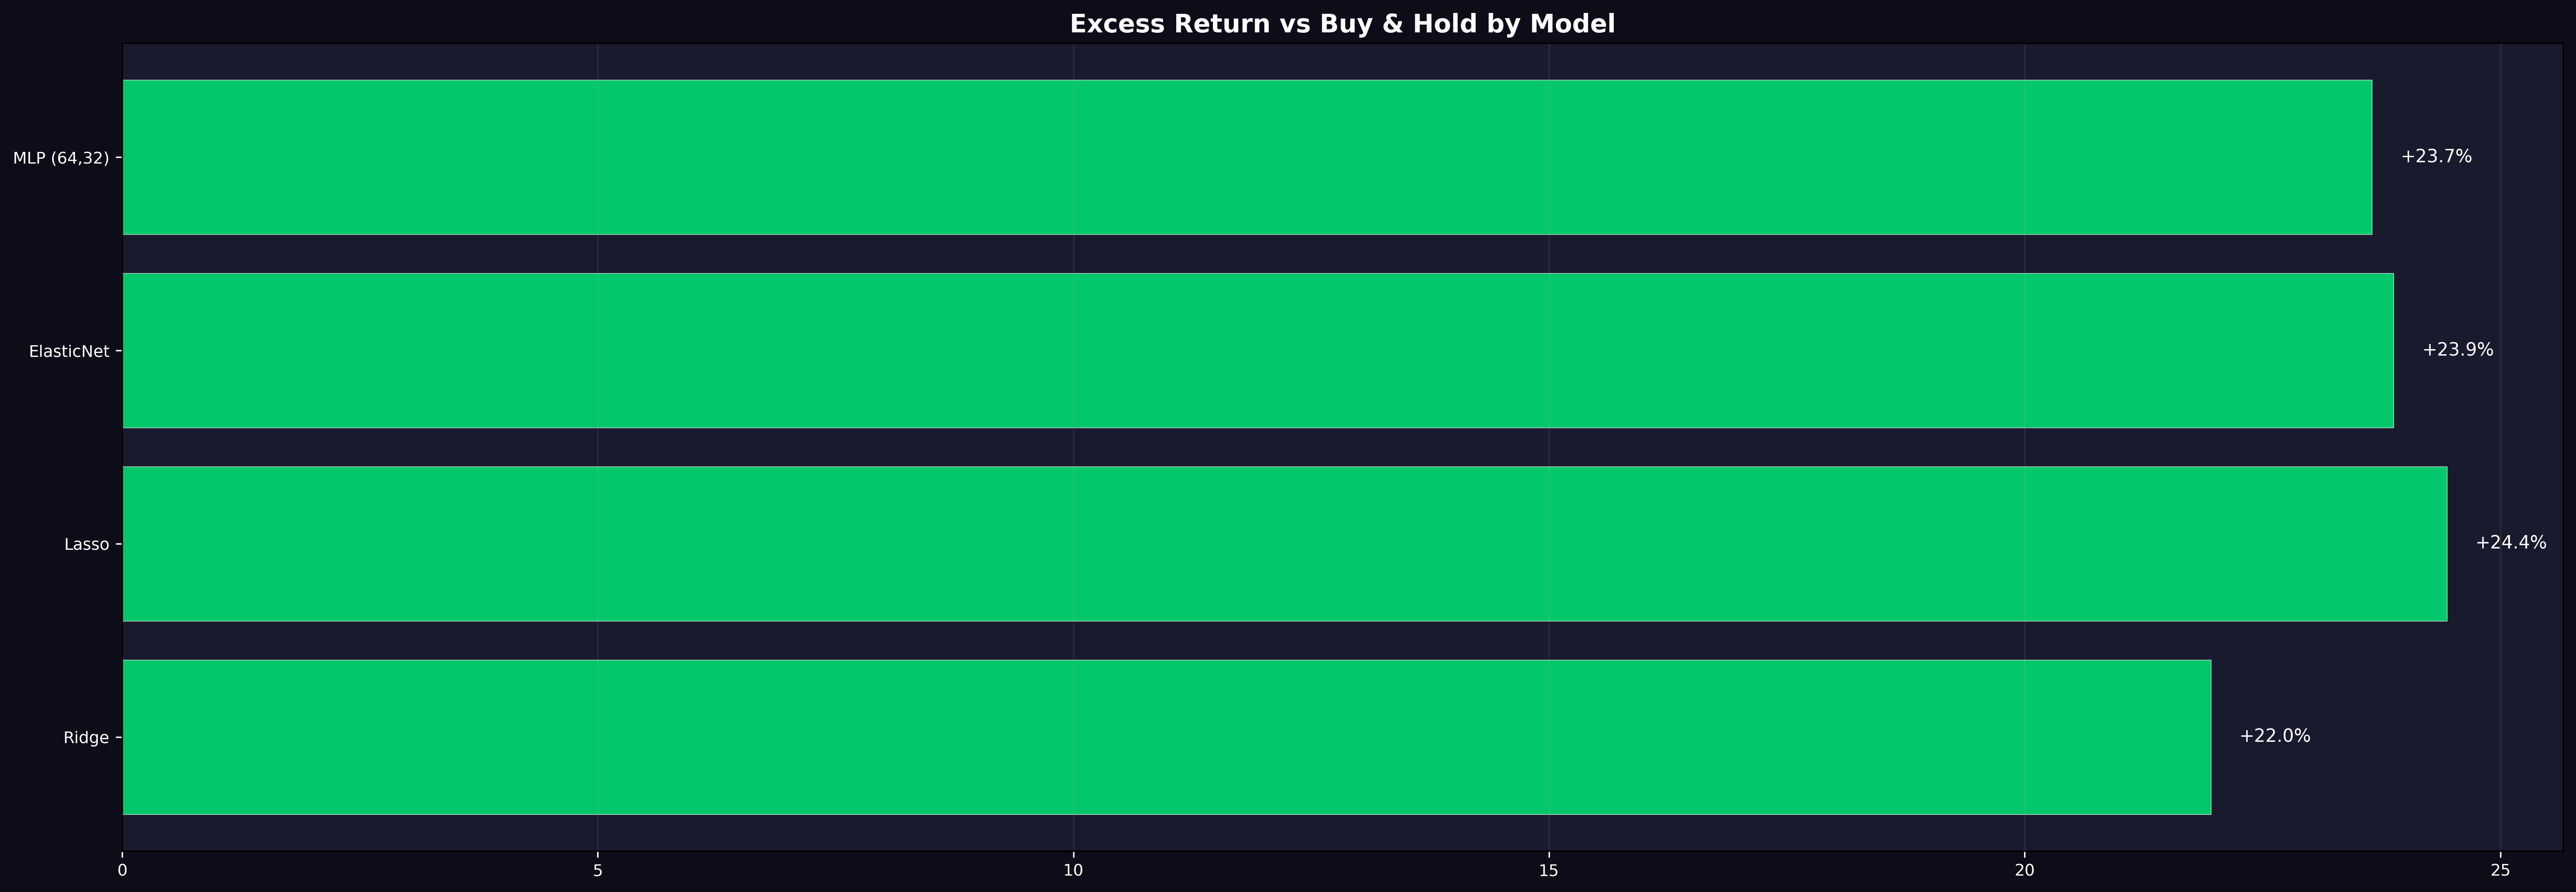
\includegraphics[width=\textwidth]{../src/strategy/trained/images/model_excess_comparison.png}
\caption{Excesso de retorno vs Buy \& Hold por modelo.}
\end{figure}

\section{Backtest Engine --- Demonstração}

O notebook \texttt{src/backtest/backtest\_engine\_demo.ipynb} demonstra todas as funcionalidades do engine com dados reais da VALE (5 anos, Yahoo Finance).

\begin{figure}[H]
\centering
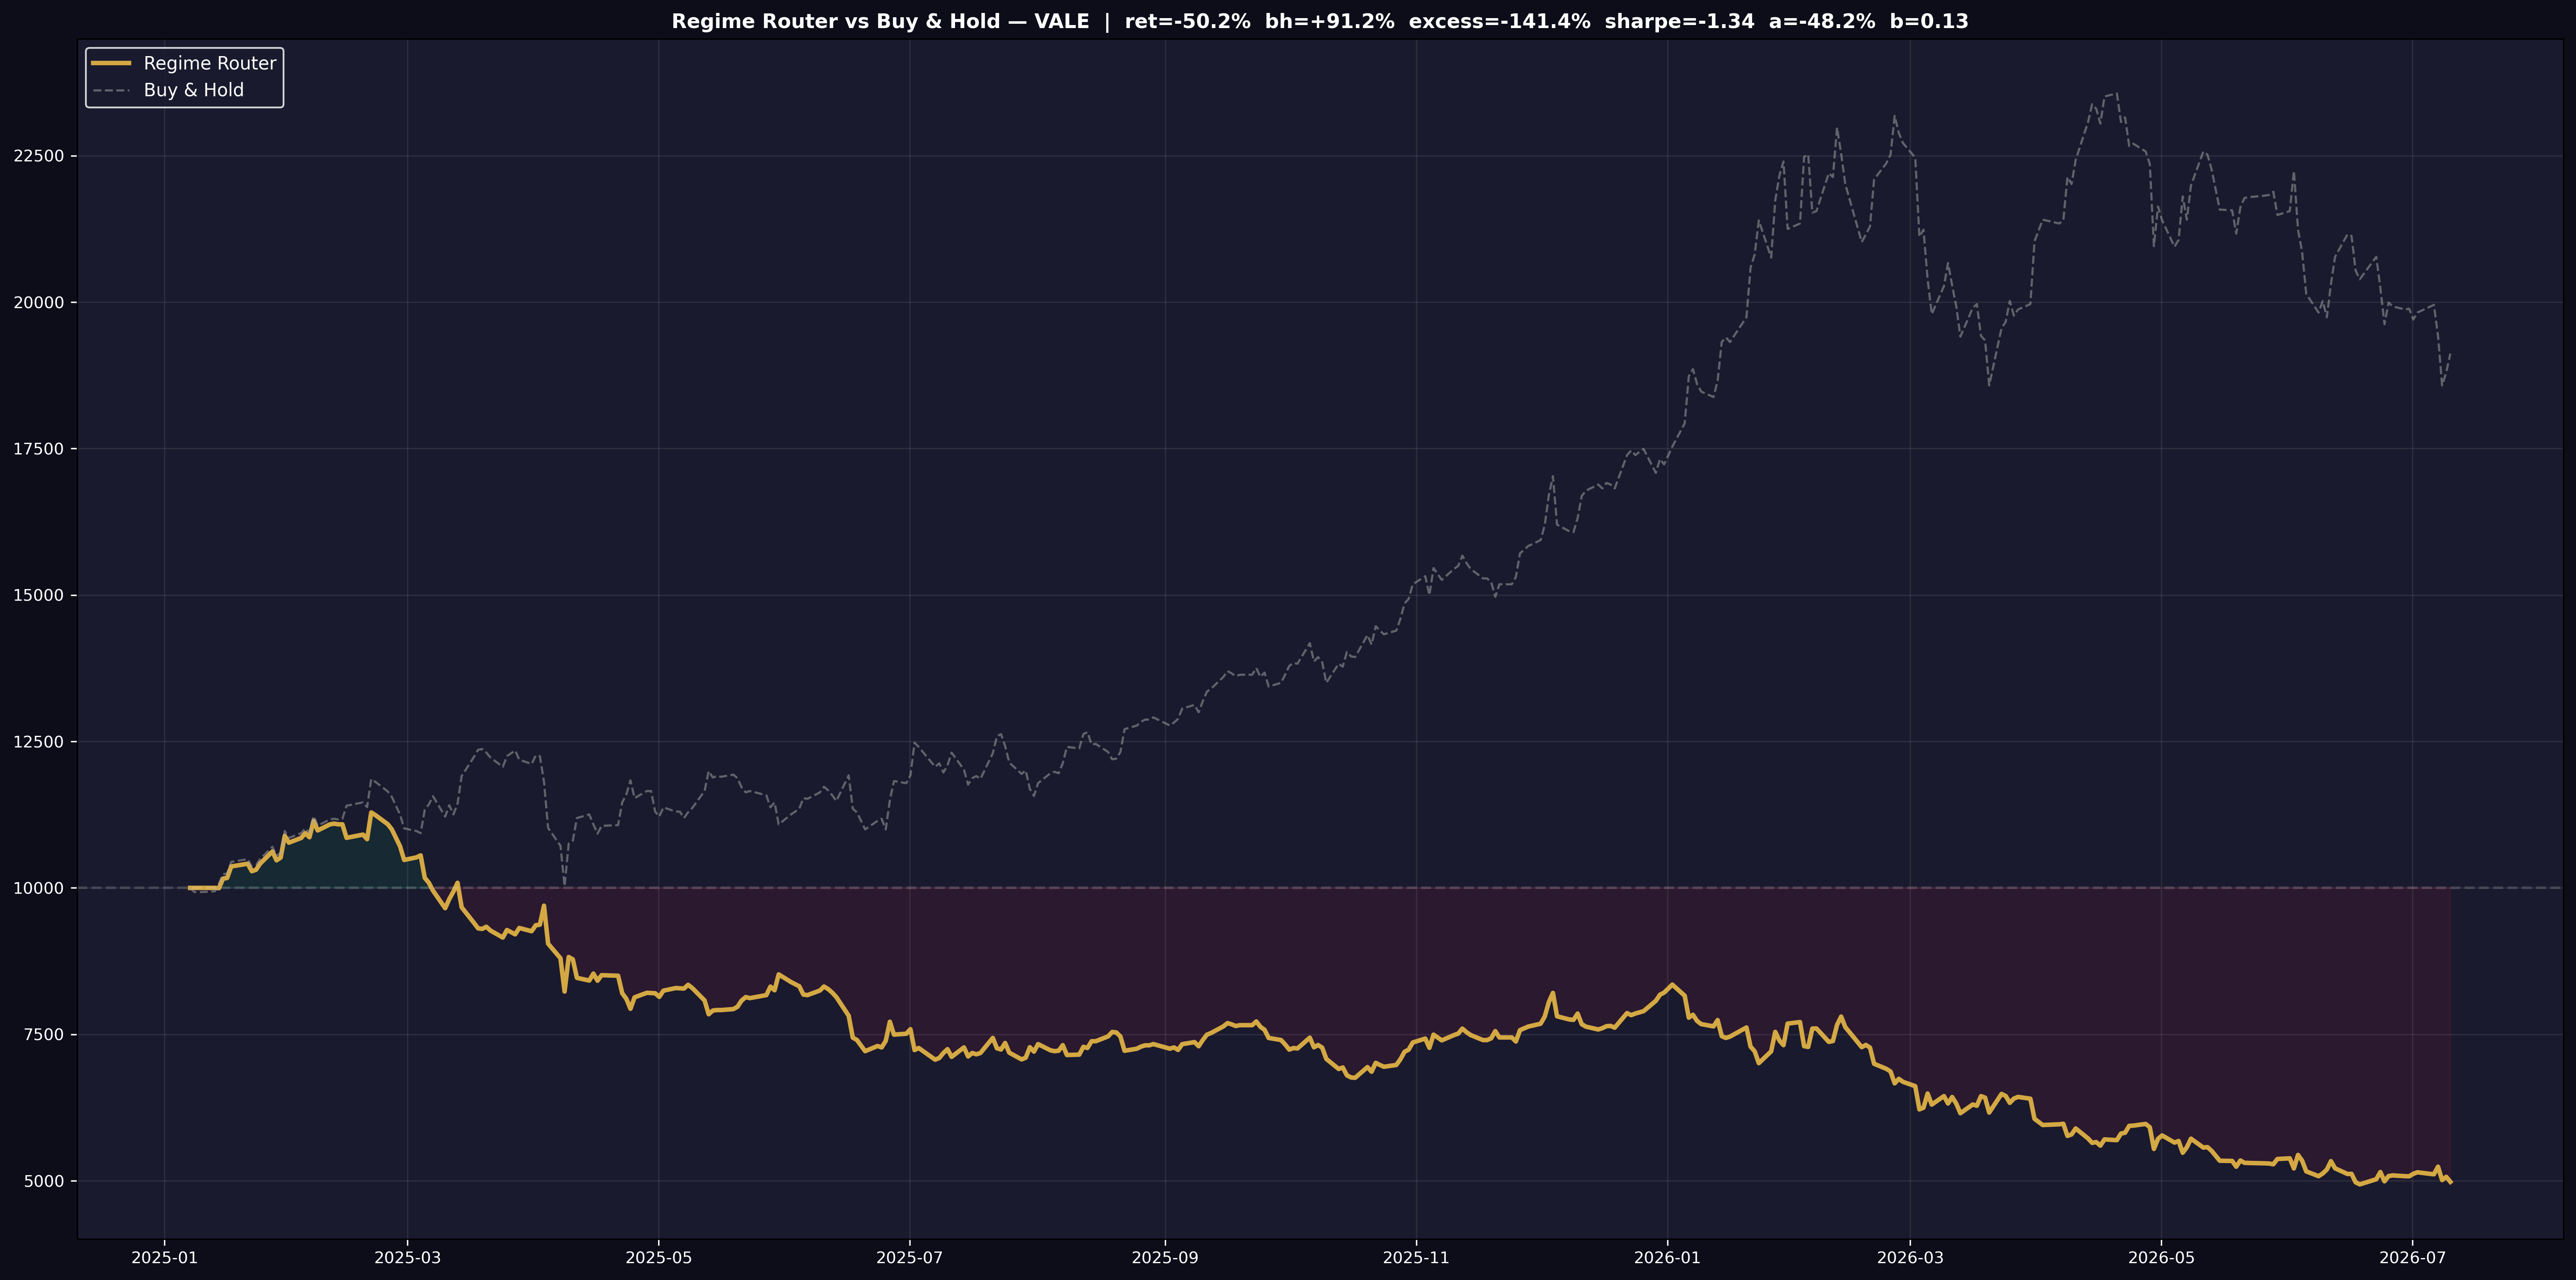
\includegraphics[width=\textwidth]{../images/backtest_demo_equity.png}
\caption{Regime Router vs Buy \& Hold --- VALE.}
\end{figure}

\begin{figure}[H]
\centering
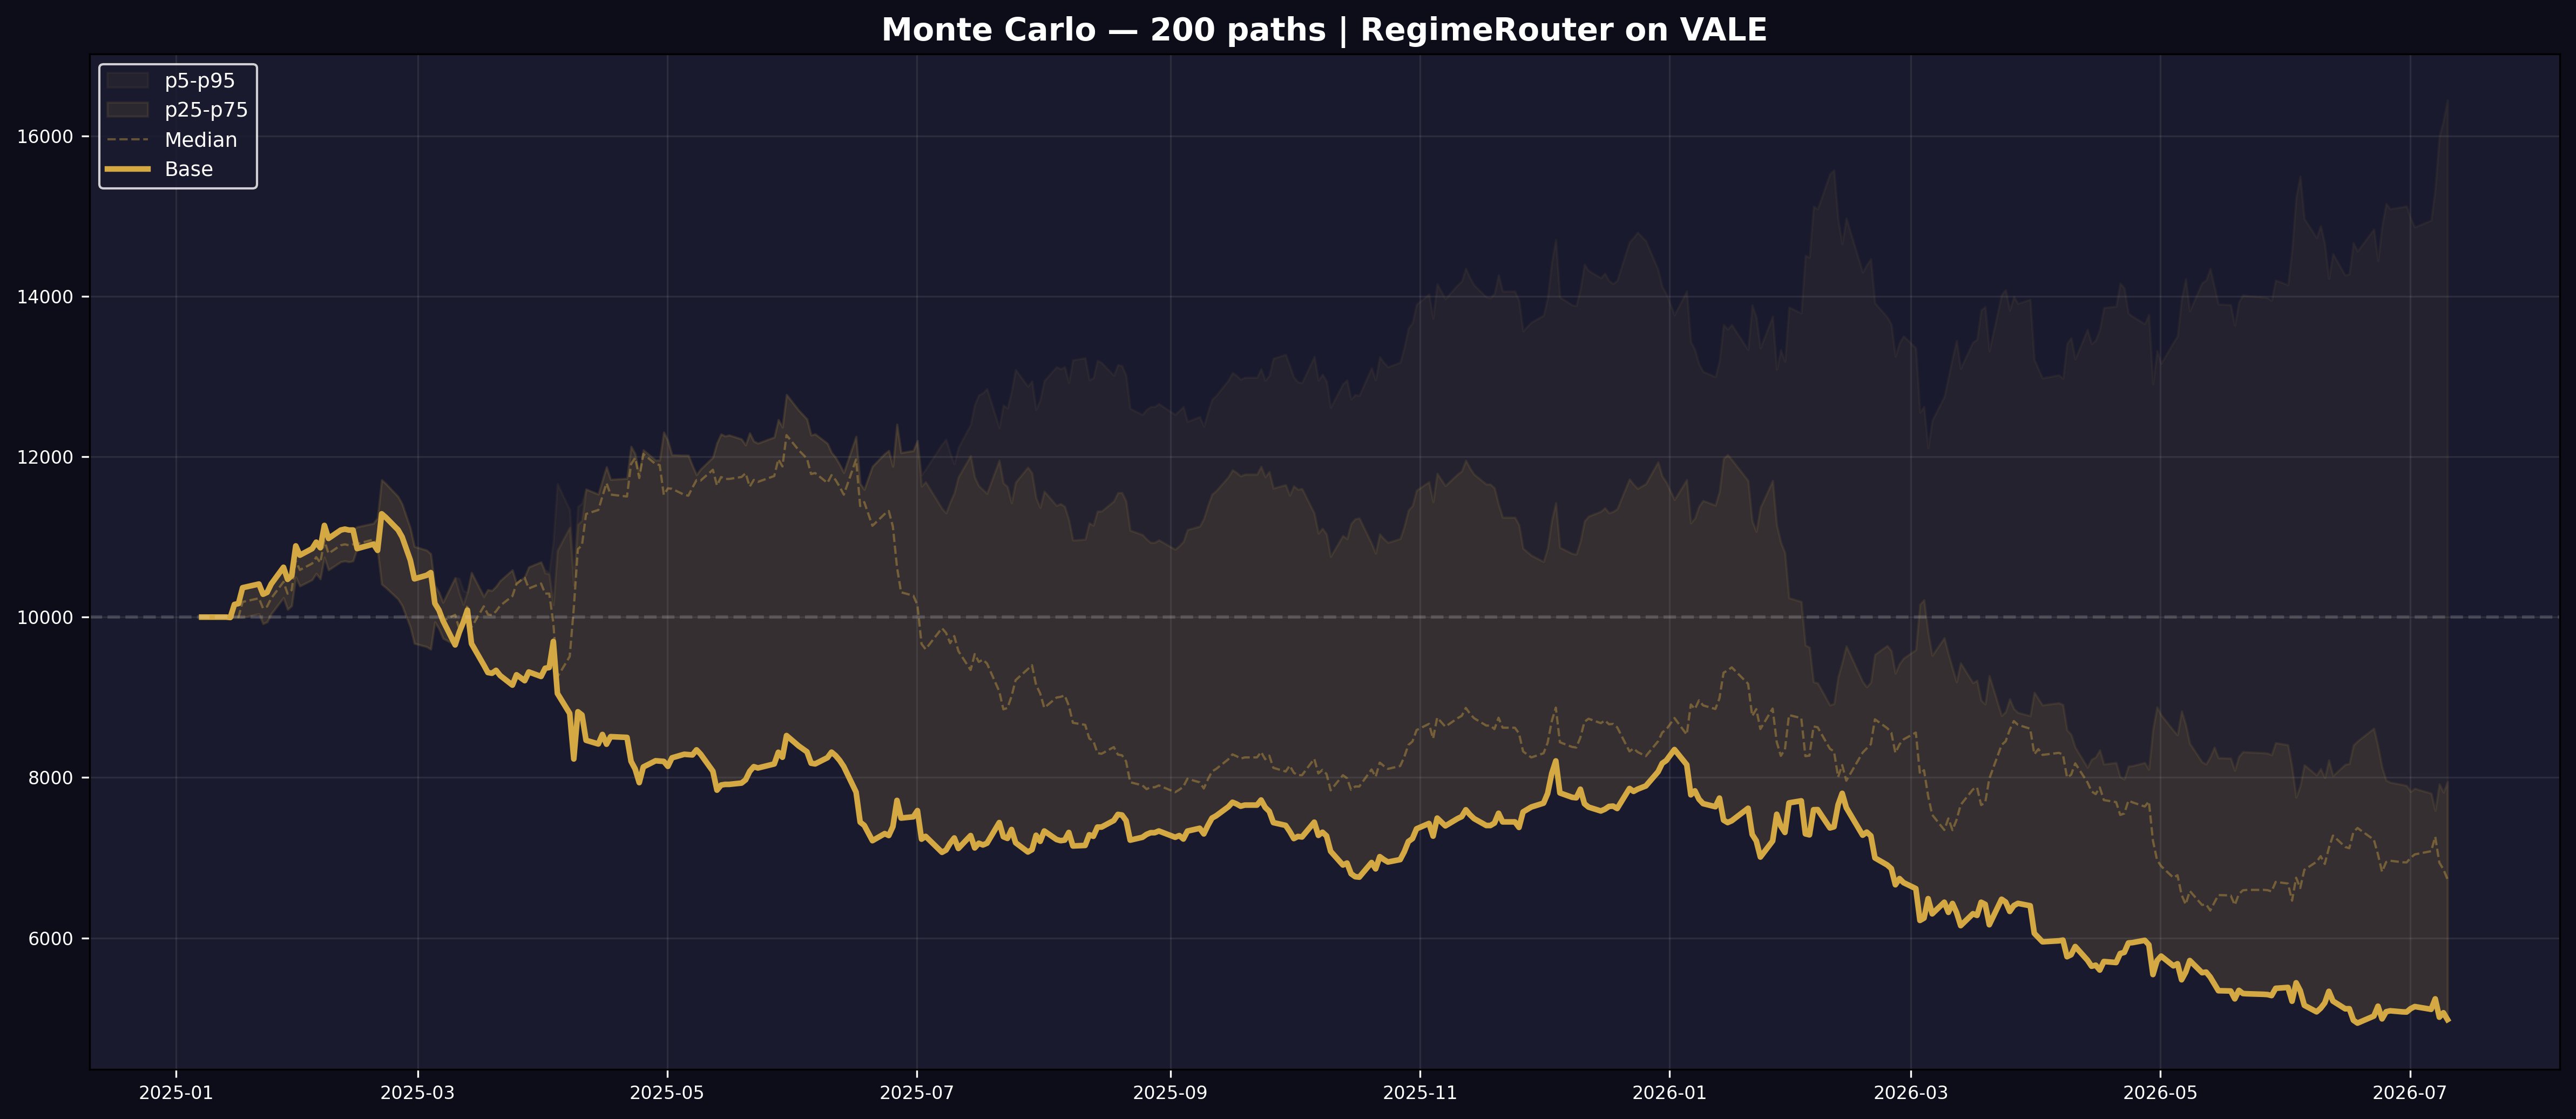
\includegraphics[width=\textwidth]{../images/backtest_demo_monte_carlo.png}
\caption{Monte Carlo: 100 simulações com noise de 8bps e delay aleatório.}
\end{figure}

\begin{figure}[H]
\centering
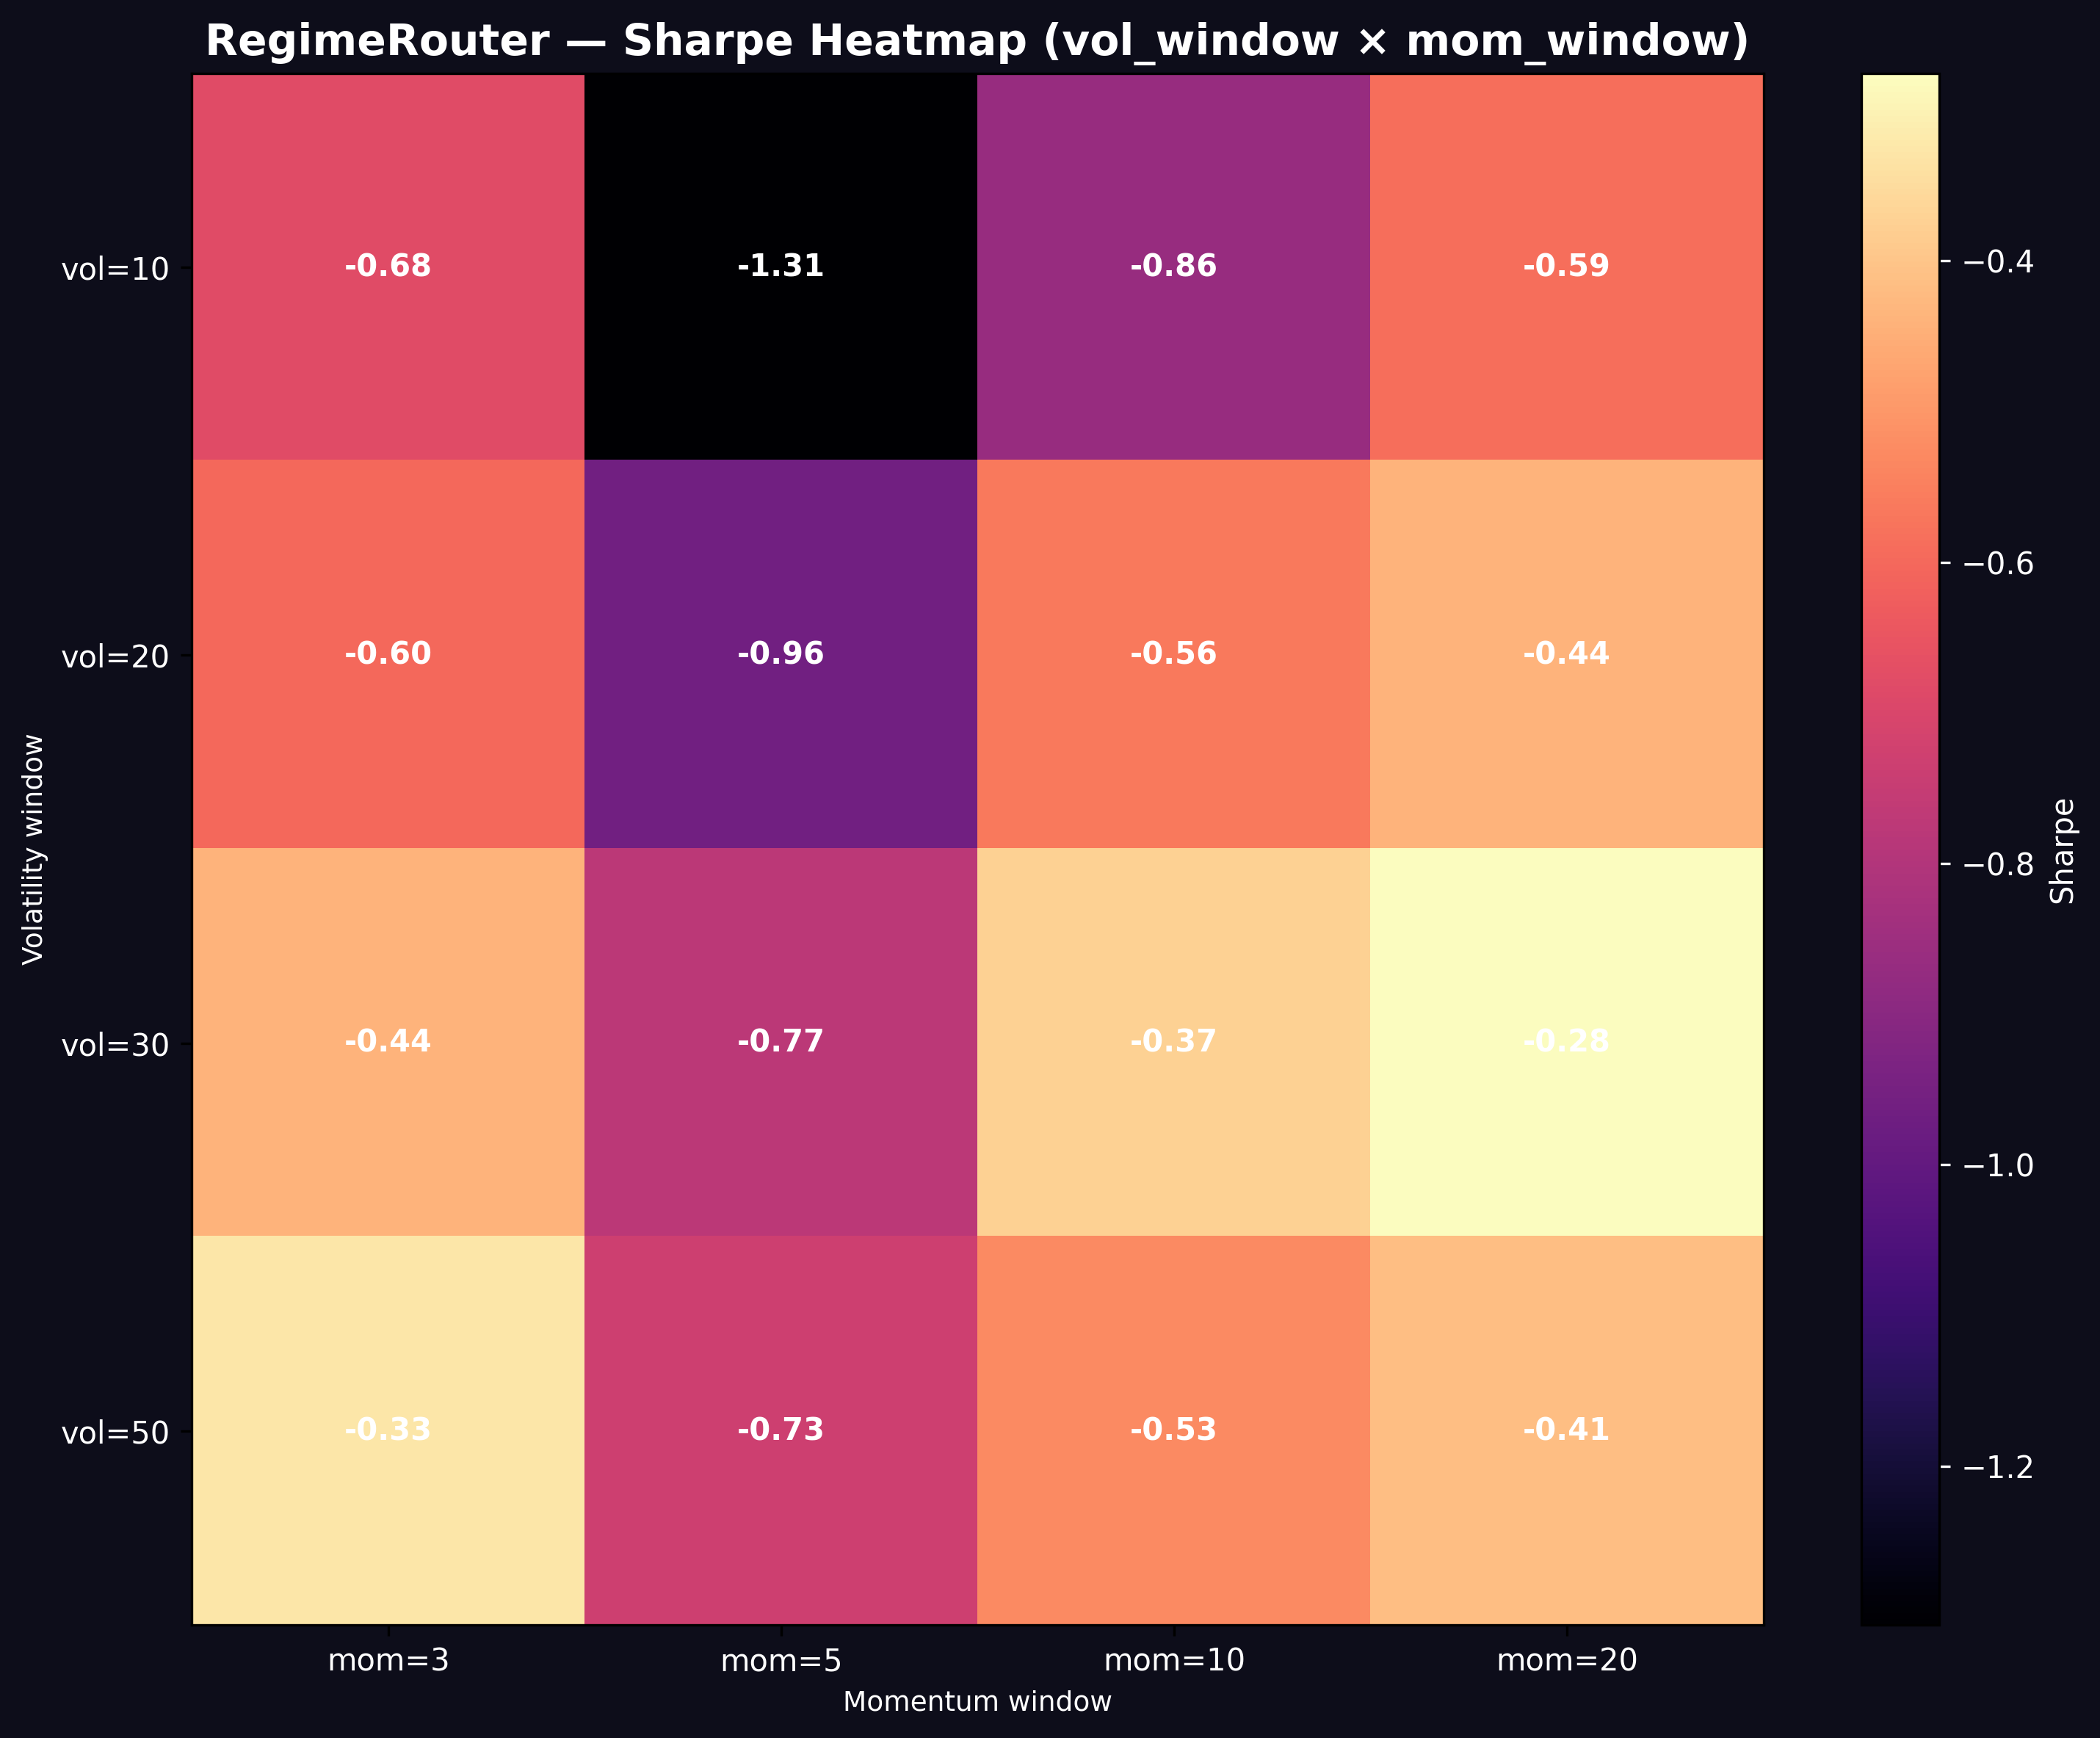
\includegraphics[width=\textwidth]{../images/backtest_demo_heatmap.png}
\caption{Heatmap de Sharpe: vol\_window $\times$ mom\_window (RegimeRouter).}
\end{figure}

\begin{figure}[H]
\centering
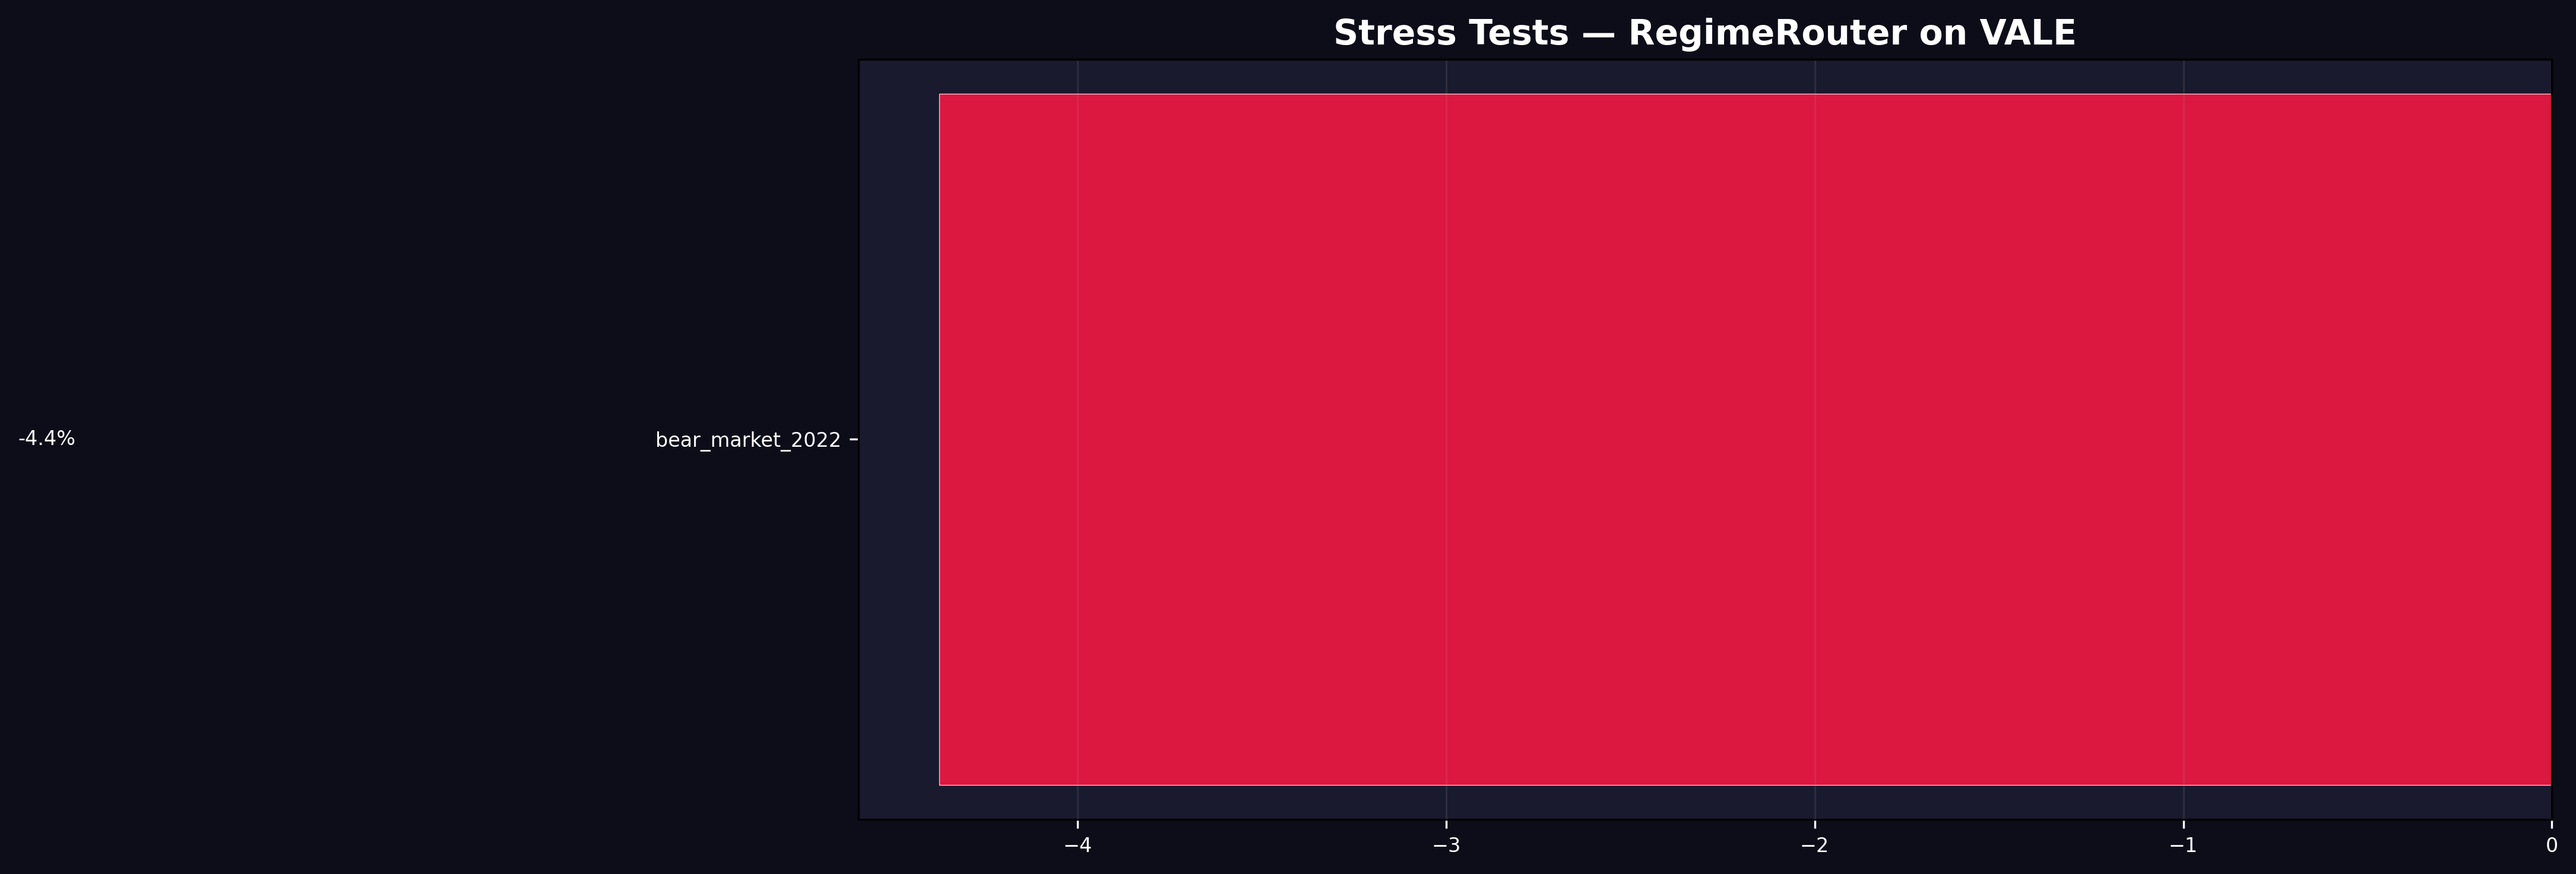
\includegraphics[width=\textwidth]{../images/backtest_demo_stress.png}
\caption{Stress tests: performance do RegimeRouter em cenários de crise.}
\end{figure}

\begin{figure}[H]
\centering
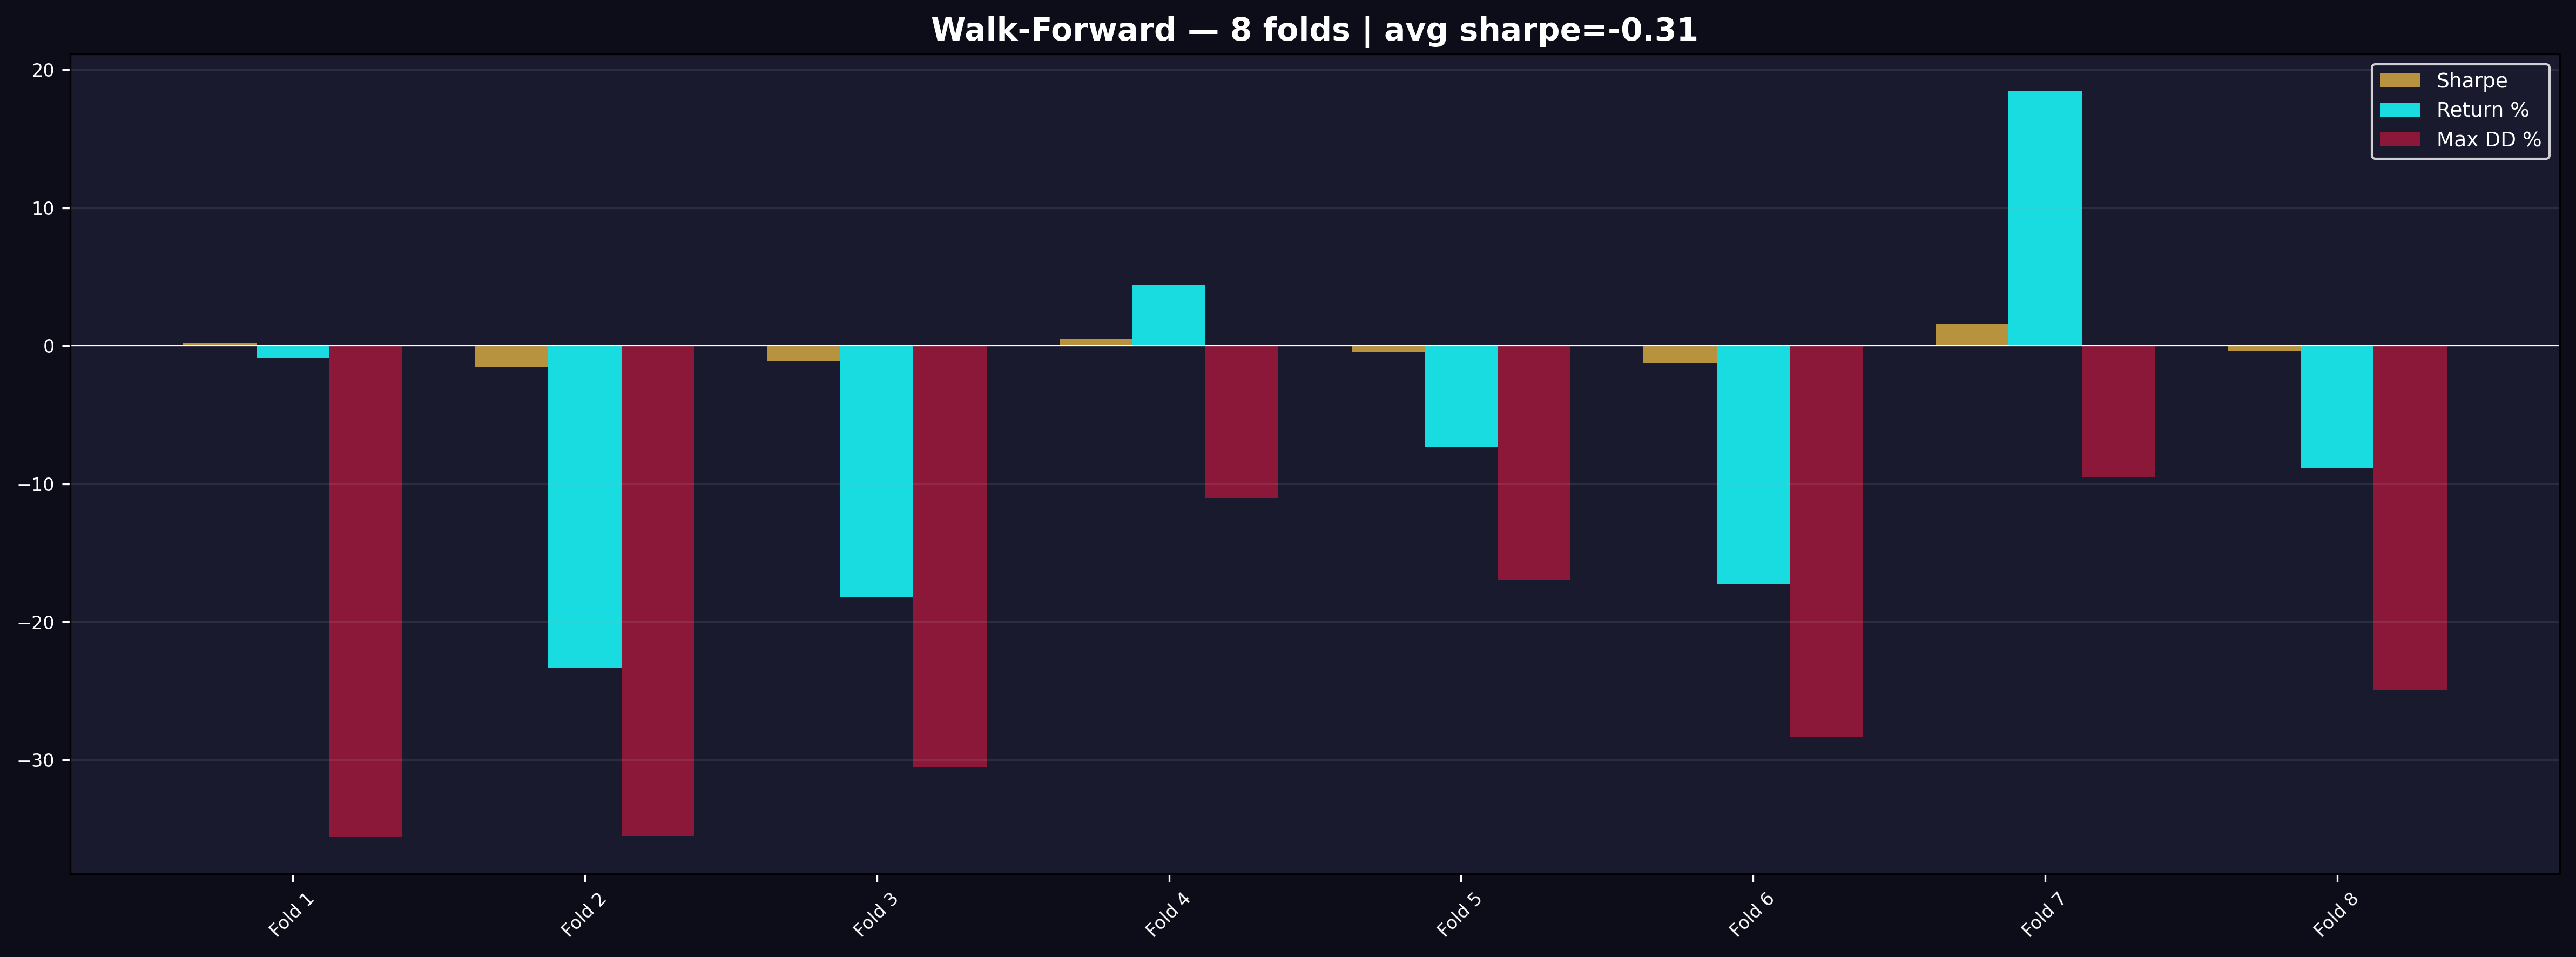
\includegraphics[width=\textwidth]{../images/backtest_demo_walkforward.png}
\caption{Walk-forward optimization: Sharpe, retorno e drawdown por fold.}
\end{figure}

\section{Conclusão}

\begin{enumerate}
    \item \textbf{Embeddings textuais geram alpha}: a estratégia S1 Hard70 obteve +28.1\% de excesso sobre buy \& hold no teste com 50 ativos, com alpha anual de +0.91\%.
    \item \textbf{Fusão multimodal funciona}: a estratégia baseada em texto supera a estratégia puramente numérica (+2.5\% de excesso vs -1.9\%).
    \item \textbf{Modelos lineares são competitivos}: Lasso e ElasticNet nos embeddings (PCA 32) produzem alpha positivo com treino rápido. MLP tem melhor correlação de treino mas não converte em alpha superior.
    \item \textbf{Pipeline de produção}: o backtest engine suporta Monte Carlo, grid search, walk-forward, stress tests e decomposição alpha/beta, pronto para expansão com dados B3.
\end{enumerate}

\section{Próximos Passos}

\begin{itemize}
    \item Treinar com dados B3 (notícias em português + séries temporais brasileiras)
    \item Implementar directional attention e alignment loss conforme paper
    \item Reinforcement learning para otimização de política de portfólio
    \item Testar com dados de crypto (DRW dataset)
    \item Black-Litterman com embeddings como views e matriz de confiança
\end{itemize}

\end{document}
